\documentclass[oneside,10pt]{swissi}

\addbibresource{4-bib/2-bib.bib}
\newcommand{\papertitle}{Verifiable Federated AI Infrastructure}
\newcommand{\papersubtitle}{Swiss compliant federated AI DLT network using Nash equilibrium and ESG metrics}

\newcommand{\papercitationauthors}{Kurz, W. and Malara, M. and Dedi{\'c}, V.}

\newcommand{\paperauthors}{%
  Walter Kurz\textsuperscript{1}%
  , Michel Malara\textsuperscript{1}%
  , Velimir Dedi{\'c}\textsuperscript{1}%
}

\newcommand{\paperaffiliations}{%
  \textsuperscript{1}Swissi Institute for AI,
  \href{mailto:kurz@swissi-ai.institute}{kurz@swissi-ai.institute};
  \href{mailto:malara@swissi-ai.institute}{malara@swissi-ai.institute};
  \href{mailto:dedic@swissi-ai.institute}{dedic@swissi-ai.institute}%
}

\newcommand{\paperdeclarationaffiliations}{%
  \begin{tabular}[t]{@{}l@{}}
    \textsuperscript{1}Swissi Institute for AI,
    \href{mailto:kurz@swissi-ai.institute}{kurz@swissi-ai.institute};
    \href{mailto:malara@swissi-ai.institute}{malara@swissi-ai.institute};
    \href{mailto:dedic@swissi-ai.institute}{dedic@swissi-ai.institute}%
  \end{tabular}%
}

\newcommand{\papercorresponding}{%
  Walter Kurz,
  \href{mailto:kurz@swissi-ai.institute}{kurz@swissi-ai.institute},
  \href{https://orcid.org/0009-0006-8045-4775}{ORCID 0009-0006-8045-4775}%
}

\newcommand{\paperfunding}{%
  This research received no external funding.%
}
\newcommand{\paperconflictsofinterest}{%
  The authors declare no conflicts of interest.%
}
\newcommand{\paperdataavailability}{%
  The data and code supporting this article are available from the corresponding author on reasonable request.%
}
\newcommand{\paperaitools}{%
  Generative AI tools were used for editorial work only, such as language editing and formatting, in accordance with international scientific standards. The authors verified the content and remain fully responsible for the article.%
}
\newcommand{\paperauthorcontributions}{%
  All authors contributed equally to this article.%
}

\providecommand{\swIncludeAuthorExamples}{}

\title{\papertitle \\[0.35em]
\normalsize \papersubtitle}

\author{{\fontsize{8}{10}\selectfont\paperauthors}\\[0.9em]
{\scriptsize\paperaffiliations}}
\date{\vspace{1.5em}}

\begin{document}
\maketitle

\begin{abstract}
Centralised AI infrastructure scales yet conflicts with latency, auditability and energy constraints. This paper sets the objective to specify and analyse a Federated AI Infrastructure that is compatible with regulatory and ESG commitments while remaining financeable for private operators. The design separates centralised training from decentralised inference and storage across five node classes (\textmu, S, M, L, XL), coordinated by a verifiable orchestrator and a permissioned DAG with asynchronous Byzantine fault tolerance. An incentive model links a size neutral availability floor to tiered workload rewards with bounded multipliers for service level attainment, ESG performance and anti concentration. Formal optimisation covers investor choice, congestion aware routing and policy instruments, yielding equilibrium conditions for mixed class participation. Compliance is developed against the Swiss regime, including token to fiat conversion through a regulated issuer under FINMA or an equivalent national authority, and alignment with EU frameworks such as GDPR and ISO~27001. Results indicate a robust mixed fleet in which L and XL nodes specialise in throughput intensive inference and ledger validation, while \textmu\ to M nodes provide edge inference, storage and continuous DAG participation. Anti concentration terms and ESG adjusted pricing sustain diversity without material efficiency loss. Implementation relies on trusted metering, on chain attestations and posted pricing calibrated to observed queues. Limitations concern parameter identification, metering fidelity and jurisdiction specific licensing.
\end{abstract}

\keywords{decentralised data centre; AI; Federated AI infrastructure; ESG; ESG-aware compute; Nash equilibrium; digital sovereignty; Swiss data regulation; tokenised infrastructure; verifiable AI services}

\bigskip

\section{Introduction}

Artificial intelligence is undergoing accelerated deployment across all sectors of the global economy. Large-scale models are being applied in industrial optimisation, financial services, public administration and national infrastructure. Governments, academic institutions and private entities are investing heavily in AI compute capacity, resulting in rapid expansion of hyperscale data centres and training infrastructure. The International Energy Agency projects that global data centre electricity demand will more than double by 2030, reaching approximately 945 TWh, with AI-optimised workloads as a primary driver. Data centres already account for 1 to 2 percent of global electricity consumption \cite{iea2025}.

This expansion is driven by geopolitical and economic imperatives but conflicts with environmental, social and governance objectives. AI infrastructure requires substantial energy inputs, produces significant thermal waste, and concentrates land use and resource control, often misaligned with local energy conditions or sustainability targets. Research from MIT reports that North American data centre power demand rose from 2,688 to 5,341 MW between 2022 and 2023. Cooling systems alone consume approximately 2 litres of water per kWh used \cite{mit2025}. The carbon footprint of training large language models can exceed 500 tons of CO\textsubscript{2}, and by 2035, annual AI-related emissions may reach 18 to 246 million tons \cite{wiki2025}.

Current data centre practices prioritise performance and centralised control over energy efficiency, auditability and regulatory decentralisation. This approach raises structural issues for ESG-compliant digital infrastructure. A recent study on sustainable cloud computing projects that, by 2025, data centres may account for up to 20 percent of global electricity demand and 5.5 percent of total emissions if uncorrected \cite{buyya2023}. The absence of standardised reporting frameworks limits transparency and restricts regulatory oversight \cite{fas2025}.

Before the commercial release of ChatGPT in November 2022, companies now leading the AI sector had publicly committed to ESG goals. Google had reached operational carbon neutrality by the mid-2000s and transitioned to 100 percent renewable energy for its data centres by 2017. Microsoft had been carbon neutral since 2012. Amazon launched its Climate Pledge in 2019, targeting net-zero emissions by 2040 and full renewable energy reliance by 2030 \cite{news20,news24,search29}.

Since late 2022, corporate strategies have shifted towards rapid scaling of generative model capabilities, with performance and market control taking precedence over sustainability. Microsoft alone reported a 168 percent increase in AI-related energy demand, alongside a 23 to 29 percent rise in emissions since 2020 \cite{news23,news21}. Industry interviews confirm that most organisations prioritised operational efficiency in AI adoption over environmental risk mitigation, with limited adherence to sustainability standards \cite{search8}. Economic studies indicate that capital allocation to AI has displaced longer-term ESG investments \cite{search18}.

This paper responds to these structural limitations by proposing a decentralised infrastructure model for AI deployment and governance. The system consists of a federation of modular data centres distributed across Swiss territory, designed to support inference execution, smart contract automation, decentralised storage and ESG-aware orchestration. Coordination is implemented through formal incentives within a tokenised and auditable framework, rather than centralised control or enforcement logic.

Switzerland provides a credible institutional and regulatory foundation for such a model. The revised Federal Act on Data Protection (FADP), in force since 1 September 2023, aligns with the European Union’s GDPR in key provisions including privacy by design and by default, expanded data subject rights, and extraterritorial application \cite{fadp2023,gdpralign2023,extraterritorial2023}. It supports international data transfers through adequacy decisions and standard contractual clauses \cite{privacyprinciples}, and its applicability to AI-driven processing has been confirmed by the Swiss Federal Data Protection and Information Commissioner \cite{fdpic2025,aiapplicability2025}. Swiss jurisdiction benefits from EU adequacy status and compliance with ISO 27001, allowing formal measurement of infrastructure performance and energy use for ESG auditability \cite{securitycertification2025}. Regulatory frameworks including the FADP, FinSA and FINMA further support sovereign governance of decentralised infrastructure and cross-border compute under legally stable conditions \cite{finmasaneutrality2024,dataregfin2025}.

\section{Related Work}

Recent studies examine the architectural separation of training, inference and orchestration across edge, fog and cloud environments. One survey analyses AI deployment across edge–cloud infrastructures, identifying polarisation effects and the absence of coordination mechanisms beyond data locality \cite{Yao2021}. Another evaluates federated learning in mobile edge networks, focusing on the resource impact of decentralised training and the role of edge-based orchestration \cite{Lim2019}. A more recent contribution introduces inference-aware orchestration, separating serving from training processes and improving model placement in hierarchical systems \cite{Lackinger2024}. Earlier work on fog computing outlines task distribution models between edge and cloud \cite{Mouradian2017}.

These contributions suggest that while federated learning addresses decentralised training and fog computing addresses workload allocation, few approaches offer verifiable orchestration across the full infrastructure. FAII addresses this by explicitly decoupling training, inference and orchestration, embedding verifiability and policy enforcement within a coordination layer designed for sovereignty and auditability.

Economic analyses explore the coexistence of fixed-price and spot markets in cloud services. Under bounded pre-emption costs, spot pricing can outperform fixed pricing in terms of provider profit and user welfare \cite{Dierks2021}. One mechanism proposes adaptive posted prices that respond to real-time utilisation, achieve optimal competitive ratios and implement congestion-sensitive pricing in online allocation \cite{Zhang2017}. A related model in the transport sector combines forward availability rights, congestion charges and real-time trading, with structural analogies to decentralised compute markets \cite{Cramton2015}. FAII diverges by enforcing corridor-bounded posted prices, capping availability and ESG multipliers, and replacing auction-based clearing with dispersion constraints.

In market theory, two-sided platforms have been modelled as weighted potential games, allowing unique Nash equilibrium selection and ensuring stability under network effects despite equilibrium multiplicity \cite{Chan2019}. Another framework addresses asymmetric platform competition through monotone best responses, proving equilibrium existence and uniqueness under parameter heterogeneity \cite{Sato2022}. FAII’s feasibility-first assignment and queue-based posted pricing implement monotone response functions under bounded multipliers and corridor constraints, consistent with these theoretical guarantees while enforcing service-level quotas and controlling dispersion.

Carbon-aware scheduling integrates emissions data, workload shifting and service reliability to optimise deployment. One framework schedules geo-distributed web services by jointly optimising latency and emissions, achieving up to 70\% CO\textsubscript{2} reduction without degrading performance \cite{Souza2024}. Another introduces a scheduler for DAG-structured data-processing jobs that minimises carbon footprint under precedence constraints, reducing emissions by up to 33\% \cite{Lechowicz2025}. A serverless scheduling approach routes functions based on real-time grid carbon intensity, lowering emissions per invocation by approximately 13\% \cite{Chadha2023}. In fixed-network settings, a carbon-aware traffic engineering scheme uses dynamic link-cost metrics incorporating router power use and grid intensity, achieving measurable improvements without hardware modification \cite{ElZahr2023}. FAII extends these approaches by embedding ESG signals as priced, bounded multipliers and applying routing bias based on attestable carbon metrics, moving beyond disclosure-based reporting.

Mechanisms for verifying outsourced computation and energy claims rely on attestation, trusted execution and cryptographic proofs. One survey examines practical deployments of confidential computing with TEEs, highlighting the role of remote attestation in detecting enclave misbehaviour in cloud systems \cite{Chen2023}. Another reviews 37 schemes combining zero-knowledge proofs, multi-party computation and verifiable computation to provide both privacy and public correctness guarantees \cite{Bontekoe2023}. Early systems for verifiable resource accounting in cloud services argue that billed resource use must reflect actual consumption under declared policies \cite{VerifiableAccounting2010}. In privacy-preserving metering, protocols using TEEs and homomorphic encryption demonstrate correctness in billing without exposing individual consumption data \cite{Rial2016}. FAII extends these concepts by requiring attestable, tamper-resistant metrics at runtime for routing and payment settlement, integrating attestation directly into the orchestration layer rather than relying on post hoc audit.

EU and Swiss data-protection frameworks impose strict obligations on data residency, accountability and controller responsibility. Public blockchains conflict with the GDPR’s right to erasure and create ambiguity in controller identification, whereas permissioned architectures support clear accountability and delete-by-design mechanisms \cite{BelenSaglam2022,Haque2021}. FAII’s orchestration layer enforces data localisation within EU or Swiss jurisdictions, reducing exposure to extraterritorial regimes such as the US CLOUD Act \cite{Wire2025,Haque2021}.

Under the EU Markets in Crypto-Assets Regulation (MiCAR, Reg 2023/1114), e-money tokens (EMTs) and asset-referenced tokens (ARTs) must remain redeemable at par value, backed by segregated high-liquidity reserves and accompanied by redemption procedures approved by a supervisory authority \cite{EBA2024,Ey2023}. FAII is designed to align structurally with these constraints by implementing token redemption through a regulated issuer, maintaining reserve coverage and assigning liability through white-paper disclosures. The model avoids interest-bearing instruments, mandates par-value redemption and provides six-month audit cycles, without asserting formal certification status.

Carbon-credit integrity depends on provenance tracking, timestamped issuance and interoperable registries to prevent double counting and over-crediting. One global meta-analysis estimates that fewer than 16\% of issued credits correspond to verifiable emissions reductions, pointing to systemic quality failures in existing registries \cite{Nature2024}. Other studies examine the use of distributed-ledger technologies and standards frameworks (e.g. ICVCM, IETA, IEEE/ISO) to enhance registry transparency through blockchain-based timestamping, unique identifiers and audit trails \cite{Baiz2024}. One platform integrates geo-fenced sensor data with on-chain smart contracts to verify the provenance of emissions events \cite{Boumaiza2024}. A cryptographic accounting model combines encryption and authentication to support jurisdiction-agnostic emissions trading with data-integrity guarantees \cite{Li2020}. FAII builds on these approaches by linking IIoT-verified, location- and time-stamped events to smart contracts, enforcing registry integrity, preventing double counting and enabling carbon-adjusted settlement.

\section{Contribution}

Existing research treats the relevant elements in isolation, namely architecture for edge AI, market mechanisms for compute, carbon aware scheduling, verifiable metering and permissioned consensus. This paper integrates these strands into a single, policy oriented infrastructure with feasibility first assignment, corridor bounded pricing, a bounded ESG multiplier grounded in attestations, and a Nash equilibrium analysis for heterogeneous node classes under jurisdictional constraints.

The paper introduces a decentralised AI infrastructure that unifies modular system design, tokenised market coordination, ESG instrumentation and formal optimisation. The contribution spans five interrelated dimensions.

The system architecture defines a federated AI cloud composed of physically distributed data centres, anchored by a central high-density training facility and supported by a nationwide network of inference and storage nodes. Deployment follows five classes (\textmu, S, M, L, XL) with standardised hardware envelopes, energy-integration interfaces and orchestration protocols. Operators can include municipalities, cooperatives, academic institutions and private actors. Training and inference are functionally decoupled to support regulatory traceability, jurisdictional control and operational scalability.

Market coordination is handled through a posted-price marketplace with a dual-token mechanism for compute allocation and energy balancing. Corridor-bounded prices, a size-neutral availability floor and capped multipliers for SLO performance, ESG and diversity align incentives while limiting volatility. Task routing follows decentralised optimisation with feasibility enforced on latency and bandwidth, and settlement is executed via smart contracts that encode service levels and verifiable payout conditions.

ESG is a binding economic signal. Timestamped and geolocated measurements of source mix, rPUE and energy-to-work feed a machine-verifiable ESG score used for routing bias and bounded multipliers. A smart-contract carbon module links IIoT events to credit minting and retirement, enabling carbon-adjusted pricing and preventing double counting through on-chain provenance.

Governance and compliance are addressed by design. The orchestrator enforces data localisation and access policies, and the token redemption path is structured to align with Swiss and EU regimes by routing redemption through a regulated issuer with segregated reserves and documented procedures. Claims are kept at the “designed to align” level rather than asserting formal certification.

Formal analysis specifies node-level optimisation under latency, energy availability, ESG obligations and token economics. Each data centre maximises a local utility function subject to verifiable constraints. Under bounded multipliers, price corridors and queue-responsive surcharges, best responses are monotone and a Nash equilibrium exists for the compute and energy sub-markets. This enables simulation of decentralised dynamics and reproducible analysis across heterogeneous legal and geographic environments.

The model supports open participation and decentralised ownership. Cities, villages and individuals can contribute certified capacity and receive revenue distributed by IIoT-based measurement and smart-contract logic. The Swiss deployment scenario serves as a regulatory prototype, with parameters adaptable to jurisdictions that require ESG-aware and sovereignty-preserving infrastructure.\\

\section{System Architecture}

The system architecture comprises two interdependent layers. The functional architecture defines the logical roles and interactions of system components. The infrastructure topology specifies the physical deployment across jurisdictions and operational environments.\\

\subsection{Functional Architecture}

The functional architecture consists of four interoperable domains: AI compute (A, CMP), decentralised data storage (B, STR), distributed ledger infrastructure (C, DLT) and orchestration (D, ORC). These components are functionally decoupled to ensure modularity, jurisdictional separation and operational independence across heterogeneous regulatory contexts. The interaction and separation of these domains are illustrated in Figure~\ref{fig:functional-architecture}.
\begin{figure}[H]
  \centering
  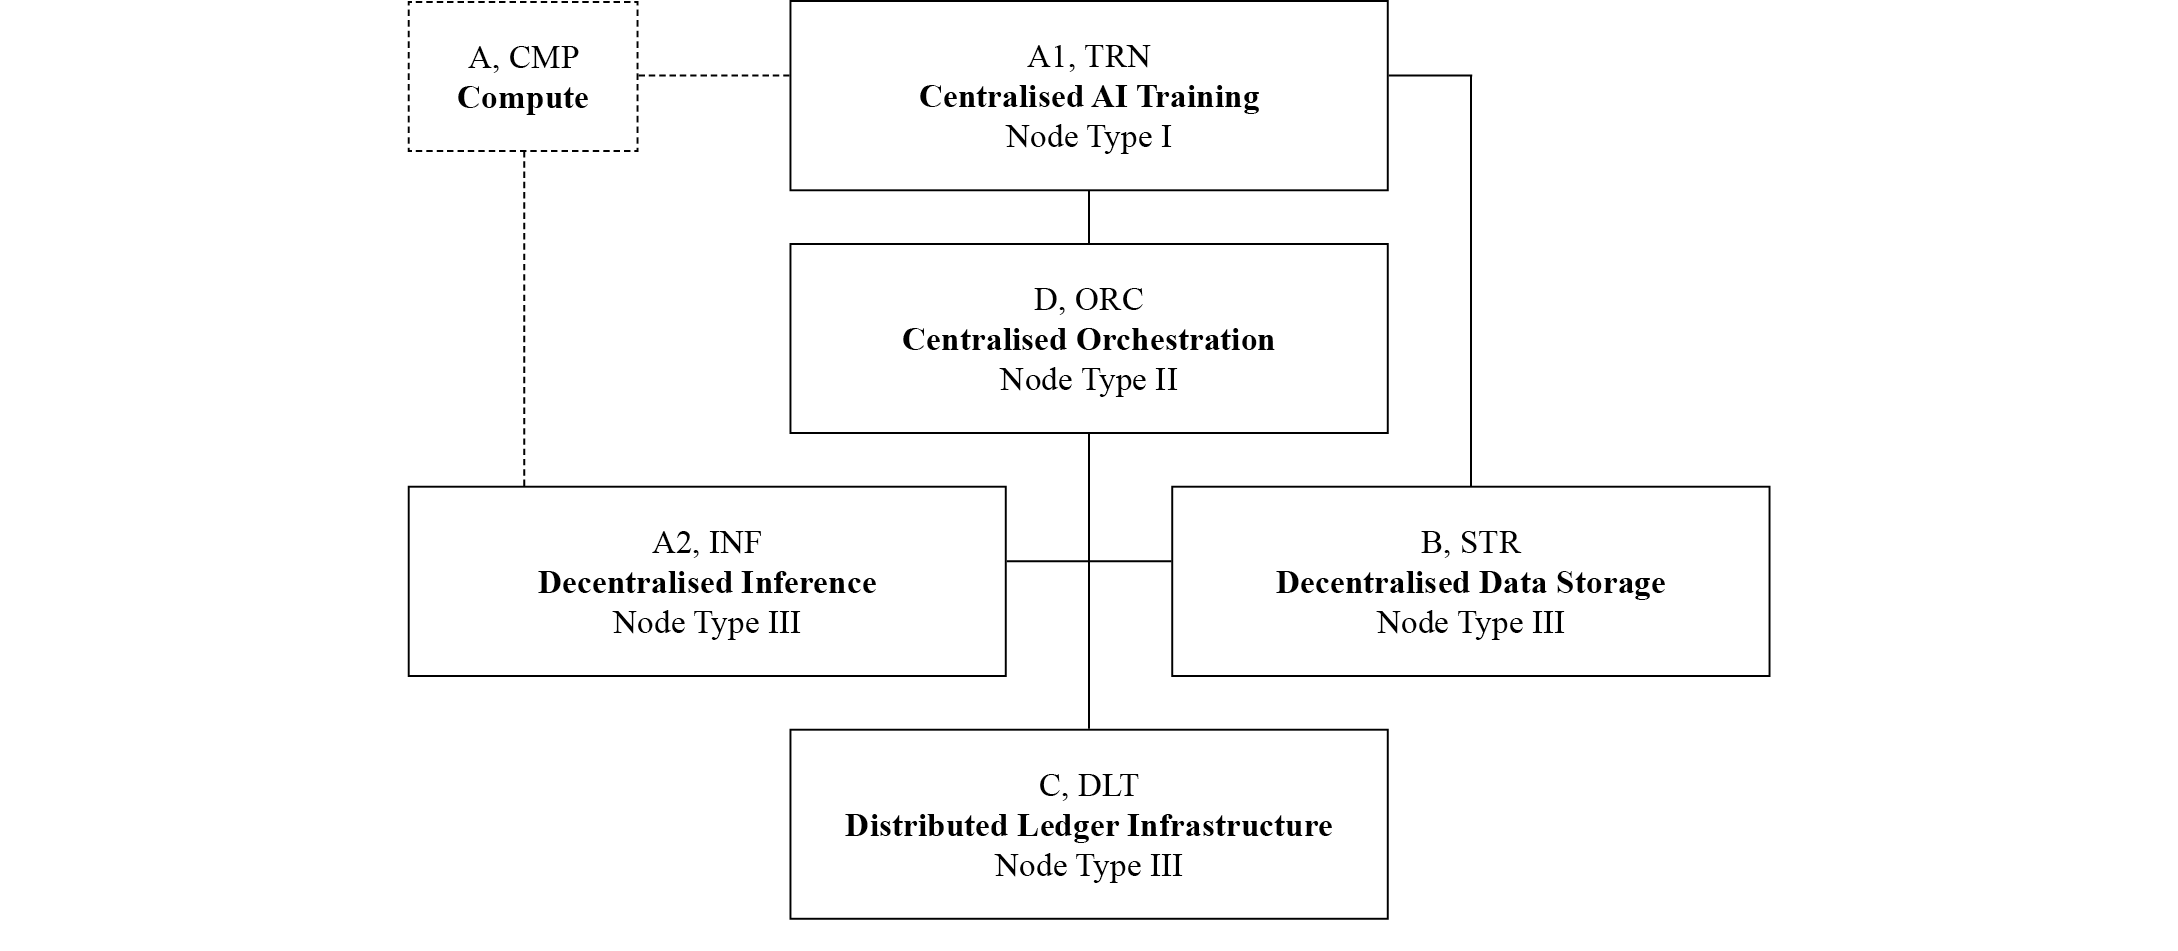
\includegraphics[width=1\textwidth]{3-assets/1-User/drwalterkurz-functional-archritecture-f1.png}
  \caption{Functional architecture of the Federated AI Infrastructure. The four system domains, comprising compute (A, CMP), storage (B, STR), ledger infrastructure (C, DLT) and orchestration (D, ORC), are assigned to three distinct node types. Compute is subdivided into centralised training (A1, TRN, Node Type I) and decentralised inference (A2, INF, Node Type III). Orchestration (D, ORC) is implemented in Node Type II. Storage (B, STR) and ledger infrastructure (C, DLT) are realised through Node Type III. Node type roles and configurations are detailed in Subsection~\ref{subsec:infrastructure-topology}.}
  \label{fig:functional-architecture}
\end{figure}

AI compute (A, CMP) is divided into two subdomains: centralised training (A1, TRN) and decentralised inference (A2, INF). Training is concentrated in a high-density facility optimised for large-model development, including pretraining, fine-tuning and reinforcement workflows. Inference is executed across geographically distributed nodes in five standardised classes, configured for energy integration, regulatory containment and latency-efficient operation. The separation of training and inference enables auditability, reduces latency externalities and permits granular control over workload distribution. Decentralised data storage (B, STR) is provided by nodes operating under certified capacity, location and availability constraints. Data are encrypted, partitioned and distributed in compliance with data residency and access governance requirements. Logical separation from compute infrastructure prevents unauthorised inference and enables independent auditing of storage operations. The distributed ledger infrastructure (C, DLT) maintains verifiable contract state, token settlement and coordination logic. It records routing instructions, ESG scoring metrics and service-level compliance under formal consensus conditions. Smart contracts execute within this layer to isolate enforcement, reduce coordination load and support sovereign governance under multi-jurisdictional constraints. System orchestration (D, ORC) is implemented by a verifiable control layer interfacing with compute, storage and ledger domains. It manages task scheduling, node registration, resource discovery and fault isolation. This layer enforces protocol-level consistency across decentralised operations and preserves coherence, auditability and regulatory traceability under functional separation.

The interaction between these domains is formalised in Equation~\eqref{eq:system-coordination}.
\begin{align}
\label{eq:system-coordination}
\mathcal{F} &: (A2, B, C) \xrightarrow{D} \mathcal{O} \\
\text{s.t.} \quad & A = A1 \cup A2,\quad A1 \cap A2 = \emptyset,\quad D \perp (A1) \nonumber
\end{align}

The function \( \mathcal{F} \) maps the operational domains, comprising decentralised inference (\( A2 \)), storage (\( B \)) and ledger infrastructure (\( C \)), into a system-wide operational state \( \mathcal{O} \), governed by the orchestration layer (\( D \)). Orchestration functions as a verifiable control interface that enforces protocol-level consistency and ensures auditability across otherwise decoupled domains. Centralised training (\( A1 \)) is excluded from this coordination logic, reflecting its independent role in large-model development. The expression \( A = A1 \cup A2 \), with \( A1 \cap A2 = \emptyset \), formalises the architectural separation of training and inference. The orthogonality condition \( D \perp (A1) \) states that orchestration operates independently of the training facility.\\

\subsection{Infrastructure Topology}
\label{subsec:infrastructure-topology}

We propose a physically distributed \textit{Federated AI Infrastructure}, structured as a jurisdictionally bounded system of interoperable node types. The topology reflects regulatory separation, functional independence and operational scalability across national infrastructure. The model is designed for sovereign deployment and supports integration with decentralised AI workloads, contract-based coordination and ESG-auditable resource governance. The relationship between functional domains and node types is shown in Figure~\ref{fig:functional-architecture}.

The infrastructure consists of three node types, each assigned distinct roles within the system architecture. Node Type I corresponds to the centralised AI training facility (A1, TRN), providing the high-density compute required for pretraining and model refinement. Node Type II implements the orchestration layer (D, ORC), responsible for coordination, routing and contract logic. Both types are centralised components and are required in every instance of the national system. They form the operational core of the architecture and are typically deployed within controlled, high-compliance environments.

The distributed ledger is implemented as a permissioned consortium DAG (Directed Acyclic Graph) using a leaderless asynchronous Byzantine Fault Tolerant (aBFT) consensus protocol. Master DAG nodes, responsible for transaction finality, ordering and cross-domain validation, are integrated into Type II. Execution-level DAG nodes, which handle contract execution and local validation, are distributed across Type III infrastructure.

Node Type III comprises all decentralised infrastructure elements, including inference nodes (A2, INF), data storage (B, STR) and operational ledger components (C, DLT). These nodes vary in physical capacity and are deployed in five standardised sizes: micro (\textmu), small (S), medium (M), large (L) and extra-large (XL). While Types I and II are fixed in number and function, Type III nodes are variable in quantity and configuration. Their distribution depends on stakeholder investment decisions, local energy availability, regulatory incentives and ESG objectives. This modularity enables each jurisdiction to calibrate its infrastructure layout to national priorities while maintaining interoperability and functional symmetry across the system.

DAG-based consensus protocols support efficient, leaderless asynchronous Byzantine fault tolerance with high throughput and fairness. One system builds on DAG-Rider and Narwhal/Tusk, combining a communication DAG with synchronous fast-path optimisation to achieve atomic broadcast without additional consensus rounds \cite{Spiegelman2022}. A recent survey classifies DAG-based distributed ledger technologies into availability-focused and consistency-focused designs, analysing trade-offs in finality, fault tolerance, and fairness \cite{Raikwar2025}. Another framework implements permissioned asynchronous DAG consensus with logical time ordering and leaderless practical BFT across consortium participants \cite{Choi2018}. FAII adopts a permissioned consortium DAG with leaderless asynchronous BFT and integrates orchestration nodes to enforce finality, sustaining throughput and fault resilience under partial synchrony.

The system-wide infrastructure can be formalised as a tuple over node types and domain assignments, as shown in Equation~\eqref{eq:infrastructure-mapping}.
\begin{align}
\label{eq:infrastructure-mapping}
\mathcal{I} &= \big( \mathcal{N}_\text{I}, \mathcal{N}_\text{II}, \mathcal{N}_\text{III} \big) \\
\text{s.t.} \quad
\mathcal{N}_\text{I} &\mapsto A1, \nonumber \\
\mathcal{N}_\text{II} &\mapsto D,\ \text{and master nodes of } C, \nonumber \\
\mathcal{N}_\text{III} &\mapsto \{A2,\ B,\ C\setminus C^*\},\quad C^* \subset C. \nonumber
\end{align}

The infrastructure is formalised as the tuple \( \mathcal{I} = \big( \mathcal{N}_\text{I}, \mathcal{N}_\text{II}, \mathcal{N}_\text{III} \big) \), where \( \mathcal{N}_\text{I} \), \( \mathcal{N}_\text{II} \) and \( \mathcal{N}_\text{III} \) denote the sets of deployed nodes of Type I, II and III, respectively. Each set is mapped to its associated functional domain. Type I nodes implement centralised AI training and are mapped to the subdomain \( A1 \). Type II nodes implement orchestration \( D \) and host the master nodes \( C^* \subset C \) of the distributed ledger infrastructure. Type III nodes support decentralised inference \( A2 \), decentralised data storage \( B \), and the remaining DAG infrastructure \( C \setminus C^* \), where \( C \setminus C^* \) denotes the execution-level ledger nodes not assigned to Type II. This formalism captures the infrastructure layout and domain separation in a system-wide view.

While Node Types I and II are deployed as single instances within each national deployment of the \textit{Federated AI Infrastructure}, their physical design must support scalable capacity. This includes vertical extension through modular upgrades and, where required, horizontal replication at the site level. During the planning and initial deployment phase, their sizing must reflect projected system traction, expected inference and coordination workloads, and jurisdiction-specific constraints on sustainable and non-renewable grid energy, commonly referred to as grey energy. Both node types are subject to an upper capacity bound determined by the maximum allocatable energy at the site, in order to prevent grid overload, maintain local infrastructure stability and support ESG-aligned deployment strategies. In this context, capacity denotes the aggregate technical potential of a node to perform its assigned function over a defined interval under nominal operating conditions. For Node Type I, this refers to sustained floating-point throughput (FLOPS) or training tokens per day, metrics standard in high-performance computing capacity planning \cite{rand2024,supercomputer2024}. For Node Type II, capacity corresponds to orchestration layer throughput, expressed as operations per second or validated control-state transitions per second, consistent with benchmarks used in orchestration and container-management frameworks \cite{straesser2023,search7}. In both cases, capacity is a function of hardware configuration, software stack efficiency, power provisioning, thermal design and compliance with operational duty cycles. It forms the basis for scaling decisions, energy budgeting and service-level estimation in infrastructure planning \cite{tierpoint2023,rand2024}. The corresponding sizing constraints for Node Types I and II are formalised in Equations~\eqref{eq:type1-scaling} and~\eqref{eq:type2-scaling}.
\begin{align}
  \text{Type I capacity:} \quad & C_{\text{TRN}} \in [C_{\text{min}}^{\text{TRN}}, C_{\text{max}}^{\text{TRN}}(E_{\text{avail}}^{\text{TRN}})] \label{eq:type1-scaling} \\
  \text{Type II capacity:} \quad & C_{\text{ORC}} \in [C_{\text{min}}^{\text{ORC}}, C_{\text{max}}^{\text{ORC}}(E_{\text{avail}}^{\text{ORC}})] \label{eq:type2-scaling}
\end{align}

Here, \( C_{\text{TRN}} \) and \( C_{\text{ORC}} \) denote the installed capacities of the central training facility (Type I) and orchestration node (Type II), respectively. Each capacity must exceed a minimum functional threshold \( C_{\text{min}}^{\cdot} \) while remaining within a jurisdiction-specific upper bound \( C_{\text{max}}^{\cdot}(E_{\text{avail}}^{\cdot}) \), determined by the permanently allocatable energy. This includes both renewable sources and transitional grey energy earmarked for AI infrastructure. These constraints ensure compliance with energy regulation and prevent destabilisation of local supply during deployment. The total installed capacity of Type III infrastructure is determined by the number and class of deployed decentralised nodes. Each node belongs to one of five standardised classes: micro, small (S), medium (M), large (L) and extra-large (XL). Node capacity is fixed per class. Stakeholders scale the system by replicating nodes within each class. The corresponding sizing constraint and class-level definitions are formalised in Equations~\eqref{eq:type3-scaling} and~\eqref{eq:type3-components}.
\begin{align}
  \text{Type III capacity:} \quad & C_{\text{III}} \in [C_{\text{min}}^{\text{III}}, C_{\text{max}}^{\text{III}}(E_{\text{avail}}^{\text{III}})] \label{eq:type3-scaling} \\
  \text{Class capacities:} \quad &
  \begin{aligned}[t]
  C_{\mu} &= n_{\mu} \cdot c_{\mu}, \quad
  C_{\text{S}} = n_{\text{S}} \cdot c_{\text{S}}, \quad
  C_{\text{M}} = n_{\text{M}} \cdot c_{\text{M}}, \\
  C_{\text{L}} &= n_{\text{L}} \cdot c_{\text{L}}, \quad
  C_{\text{XL}} = n_{\text{XL}} \cdot c_{\text{XL}}, \quad
  C_{\text{III}} = C_{\mu} + C_{\text{S}} + C_{\text{M}} + C_{\text{L}} + C_{\text{XL}}
  \end{aligned}
  \label{eq:type3-components}
\end{align}

Here, \( C_{\text{III}} \) denotes the total installed capacity of Type III infrastructure. The lower bound \( C_{\text{min}}^{\text{III}} \) corresponds to minimum viable operation. The upper bound \( C_{\text{max}}^{\text{III}}(E_{\text{avail}}^{\text{III}}) \) reflects the maximum permitted capacity under ESG-aligned energy allocation. The class-level components are defined by fixed node capacities \( c_{i} \) and the number of deployed nodes \( n_{i} \), for each class \( i \in \{\mu, \text{S}, \text{M}, \text{L}, \text{XL}\} \).

Unlike Node Types I and II, which scale through capacity extension within a fixed node instance, Type III infrastructure scales horizontally by replicating nodes across the defined classes. Each Type III node operates at a fixed capacity determined by its class and is not internally extendable.

When additional capacity is required, stakeholders may provision new nodes in any of the five standardised sizes. This scaling logic preserves operational granularity, simplifies energy budgeting and supports incremental expansion strategies tailored to local constraints and stakeholder resources.

Each Node Type III instance integrates all operational subsystems required for decentralised participation, including AI inference execution (A2, INF), certified data storage (B, STR) and distributed ledger operations (C, DLT). This composite design ensures that each deployed node can independently execute inference tasks, host partitioned and encrypted data, and validate or execute smart contracts within the permissioned DAG infrastructure. Embedding all three functional domains in a unified physical unit enables modular deployment, localised resilience and protocol-level interoperability across geographically distributed infrastructure.\\

\subsubsection{Node Class Functions and Size Differentiation}
\label{subsubsec:typeIII-differentiation}

The current model defines Node Type~III in five physical sizes: micro (\textmu), small (S), medium (M), large (L) and extra-large (XL). Each node class integrates the full operational stack—decentralised inference (A2, INF), data storage (B, STR) and ledger functions (C, DLT)—and is in principle eligible to perform any system task. This raises the question of whether physical node size should imply functional differentiation or whether all nodes should retain identical eligibility within orchestration logic.

Two configurations are possible. In a uniform model, all classes implement the same functional capabilities. Task allocation remains size-agnostic, with orchestration decisions based solely on availability and compliance. This approach simplifies protocol logic and promotes egalitarian participation but may produce suboptimal outcomes, particularly if small nodes are assigned compute-intensive inference or contract execution workloads.

A differentiated model assigns functional focus by node size. Micro and small nodes may prioritise low-latency edge inference and local storage, while L and XL nodes could be allocated to compute-intensive inference or high-throughput ledger validation. This configuration enables performance optimisation, more efficient energy allocation and structured incentives. Stakeholders could select investment tiers based on workload contribution and monetisation logic. Both models present viable trade-offs. Uniformity maximises system redundancy and simplifies governance. Differentiation introduces economic signalling, strategic investment logic and supports workload specialisation, potentially improving efficiency and stakeholder returns. The architectural choice affects task distribution as well as the convergence properties of decentralised coordination models such as Nash equilibrium under constrained resources. To formalise the economic reasoning behind Type~III participation and orchestration in the \textit{Federated AI Infrastructure}, we define a capacity allocation and service model. The objective is to characterise investor class selection, orchestration-induced workload distribution, and the resulting equilibrium under energy, reliability and compliance constraints.

Let the set of Type~III classes be \(\mathcal{C} = \{\text{\textmu}, \mathrm{S}, \mathrm{M}, \mathrm{L}, \mathrm{XL}\}\). For each class \(i \in \mathcal{C}\), let \(n_i \in \mathbb{N}\) denote the number of deployed nodes, \(c_i > 0\) the fixed per-node capacity, and \(\Sigma_i = n_i\,\sigma_i\) the effective service capacity, where \(\sigma_i > 0\) is the verified per-node service rate. System tasks arrive at rate \(\lambda > 0\). The orchestration layer selects a routing share \(\phi_i \in [0,1]\) with \(\sum_{i \in \mathcal{C}} \phi_i = 1\). Define class utilisation as
\begin{align}
u_i \;=\; \frac{\phi_i\,\lambda}{\Sigma_i}\,.
\label{eq:utilisation}
\end{align}
Service-level success is given by \(s_i = s_i(u_i, \tau_i, r_i) \in [0,1]\), where \(\tau_i\) and \(r_i\) denote latency and reliability parameters, respectively. The function \(s_i(\cdot)\) is non-increasing in \(u_i\) and non-decreasing in \(\tau_i\) and \(r_i\). The verified work performed by class \(i\) is
\begin{align}
\mathcal{V}_i \;=\; \phi_i\,\lambda\, s_i(u_i, \tau_i, r_i)\,.
\label{eq:verified-work}
\end{align}

Protocol rewards are paid per unit of verified work at base rate \(p>0\) with optional class multiplier \(m_i\ge 0\). Energy consumption for class \(i\) is decomposed as \(e_i=e_i^{\mathrm{idle}}+e_i^{\mathrm{dyn}}(\mathcal{V}_i)\), where \(e_i^{\mathrm{dyn}}(\cdot)\) is non decreasing. Let \(\kappa_e>0\) denote the effective energy price per unit at site power usage effectiveness. Let \(o_i\ge 0\) be non energy operating costs, \(\kappa_o>0\) the cost conversion factor, \(\delta\ge 0\) the amortisation rate, and \(\mathrm{capex}_i>0\) the class specific investment. Penalties \(\ell_i=\ell_i(u_i)\ge 0\) apply for SLO violations or consensus faults and are non decreasing in \(u_i\).

Expected net return for operating a node of class \(i\) is
\begin{align}
R_i \;=\; p\,m_i\,\mathcal{V}_i \;-\; \kappa_e\,e_i \;-\; \kappa_o\,o_i \;-\; \varphi\,\ell_i \;-\; \delta\,\mathrm{capex}_i\,,
\label{eq:return}
\end{align}
where \(\varphi>0\) scales penalties. Risk sensitive investors with absolute risk parameter \(\rho\ge 0\) maximise mean–variance utility
\begin{align}
U_i \;=\; \mathbb{E}[R_i] \;-\; \rho\,\mathrm{Var}(R_i)\,.
\label{eq:mean-variance}
\end{align}

Each node faces site constraints for energy, bandwidth, availability, certification and carbon
\begin{align}
e_i \le E_{\mathrm{loc}},\qquad
b_i \le B_{\mathrm{loc}},\qquad
a_i \ge a_{\min},\qquad
\theta_i \in \Theta_{\mathrm{cert}},\qquad
\mathrm{CO2}_i \le \Gamma_{\mathrm{cap}}\,.
\label{eq:local-constraints}
\end{align}
Tasks may require minimum hardware features. Let \(\chi_i\in\{0,1\}\) denote eligibility for a given task class, with \(\chi_i=1\) if class \(i\) satisfies the requirement. The verified work in \eqref{eq:verified-work} is then understood conditional on \(\chi_i=1\).

Given orchestration policy \(\phi=(\phi_i)_{i\in\mathcal{C}}\), rewards \((p,m_i)\) and deployed supply \(n=(n_i)_{i\in\mathcal{C}}\), a profit maximising, risk sensitive stakeholder chooses a class \(i\in\mathcal{C}\) to maximise
\begin{align}
\max_{i\in\mathcal{C}}\quad & U_i \quad \text{s.t.}\quad \eqref{eq:utilisation}\text{--}\eqref{eq:local-constraints}\,.
\label{eq:investor-problem}
\end{align}
Risk neutral behaviour is obtained by setting \(\rho=0\) in \eqref{eq:mean-variance}.

The orchestration layer sets \(\phi\) and pricing instruments \((p,m_i)\) to achieve policy objectives subject to feasibility and market clearing. Let welfare be the verified work net of energy and externalities, with optional diversity regularisation to avoid concentration. For a weight \(\eta\ge 0\) on concentration and convex regulariser \(\Psi(\phi)\), define
\begin{align}
\max_{\phi,(p,m_i)}\quad & \underbrace{\sum_{i\in\mathcal{C}} \big(p\,m_i\,\mathcal{V}_i - \kappa_e\,e_i \big)}_{\text{net verified work}} \;-\; \eta\,\Psi(\phi) \\
\text{s.t.}\quad & \sum_{i\in\mathcal{C}}\phi_i = 1,\quad \phi_i \ge 0,\quad \text{\eqref{eq:utilisation}\text{--}\eqref{eq:local-constraints}},\quad \text{eligibility } \chi_i=1\ \text{when required}\,.
\label{eq:orchestrator-problem}
\end{align}
A common choice is \(\Psi(\phi)=\sum_{i}\phi_i^2\), which penalises concentration and preserves decentralisation.

Routing shares interact with congestion through \eqref{eq:utilisation}. For a given \(i\), assume \(s_i(u_i,\tau_i,r_i)\) is continuously differentiable and strictly decreasing in \(u_i\) on \([0,1)\). The marginal verified work with respect to \(\phi_i\) is
\begin{align}
\frac{\partial \mathcal{V}_i}{\partial \phi_i}
\;=\; \lambda\,s_i(u_i,\tau_i,r_i) \;+\; \phi_i\,\lambda\,\frac{\partial s_i}{\partial u_i}\,\frac{\partial u_i}{\partial \phi_i}
\;=\; \lambda\,s_i \;+\; \phi_i\,\lambda\,\frac{\partial s_i}{\partial u_i}\,\frac{\lambda}{\Sigma_i}\,,
\label{eq:marginal-verified}
\end{align}
which is strictly less than \(\lambda\,s_i\) when \(\partial s_i/\partial u_i<0\). Congestion reduces marginal gains from additional routing to saturated classes.

An equilibrium is a tuple \((\phi^\star,(p^\star,m^\star_i),n^\star)\) such that, given \((\phi^\star,(p^\star,m^\star_i))\), each stakeholder’s class choice solves \eqref{eq:investor-problem} and leads to the supply vector \(n^\star\). Given \(n^\star\), the orchestration problem \eqref{eq:orchestrator-problem} yields \(\phi^\star,(p^\star,m^\star_i)\). Free entry or participation conditions can be imposed as \(U_i\ge 0\) for active classes and \(U_i\le 0\) otherwise.

Return equalisation per unit of capital or energy under size neutral orchestration requires stringent assumptions. Let \(\bar R_i\) denote return per unit of capital \(K_i\) or per unit of energy \(\mathcal{E}_i\). Suppose \(m_i=1\) for all \(i\), \(s_i(\cdot)\equiv \bar s\) independent of \(i\), \(e_i^{\mathrm{dyn}}(\mathcal{V}_i)=\alpha\,\mathcal{V}_i\) with a common \(\alpha>0\), \(o_i\) and \(\mathrm{capex}_i\) linear in capacity with common coefficients, and no discrete eligibility constraints. Then
\begin{align}
\bar R_i \;=\; \frac{R_i}{K_i}\;\; \text{or} \;\; \frac{R_i}{\mathcal{E}_i} \;=\; \text{constant across } i \quad \Longleftrightarrow \quad \frac{\phi_i\,\lambda}{\Sigma_i}=\text{constant across } i\,,
\label{eq:equalisation}
\end{align}
which requires equal utilisation \(u_i\) across classes by \eqref{eq:utilisation}. Any deviation from linear costs, identical success probabilities or equal utilisation breaks equalisation. Scale economies in capex, class specific PUE, eligibility thresholds and non linear penalties \(\ell_i(u_i)\) induce persistent wedges in \(\bar R_i\).

The reward sensitivity to energy price satisfies
\begin{align}
\frac{\partial R_i}{\partial \kappa_e} \;=\; -\,e_i \;<\; 0\,,
\qquad
\frac{\partial R_i}{\partial p} \;=\; m_i\,\mathcal{V}_i \;>\; 0\,.
\label{eq:comparative-statics}
\end{align}
Congestion reduces marginal returns through \(\partial R_i/\partial \phi_i = p\,m_i\,\partial \mathcal{V}_i/\partial \phi_i - \kappa_e\,\partial e_i/\partial \phi_i - \varphi\,\partial \ell_i/\partial \phi_i\), with \(\partial \mathcal{V}_i/\partial \phi_i\) given by \eqref{eq:marginal-verified}. Risk aversion lowers class attractiveness as
\begin{align}
\frac{\partial U_i}{\partial \rho} \;=\; -\,\mathrm{Var}(R_i) \;\le\; 0\,,
\label{eq:risk}
\end{align}
which shifts participation away from classes with volatile rewards or energy costs.

Size neutral pricing with \(m_i\equiv 1\) and \(\eta=0\) in \eqref{eq:orchestrator-problem} can still generate effective size bias when \(s_i(\cdot)\), \(\mathrm{PUE}_i\) or \(\mathrm{capex}_i\) exhibit class dependent scale effects. To internalise policy goals for decentralisation, carbon or latency, the orchestration layer can implement class multipliers \(m_i=m_i(\text{ESG}_i,\tau_i,r_i)\) and a convex concentration term with \(\eta>0\). The first order condition for \(\phi_i\) under an interior solution satisfies
\begin{align}
p\,m_i\,\frac{\partial \mathcal{V}_i}{\partial \phi_i} \;-\; \kappa_e\,\frac{\partial e_i}{\partial \phi_i} \;-\; \varphi\,\frac{\partial \ell_i}{\partial \phi_i} \;-\; \eta\,\frac{\partial \Psi}{\partial \phi_i} \;=\; \nu\,,
\label{eq:KKT-routing}
\end{align}
with \(\nu\) the Lagrange multiplier on \(\sum_i \phi_i=1\). Class specific \(m_i\) should be applied only where efficiency gains from scale are demonstrated by higher \(\partial \mathcal{V}_i/\partial \phi_i\) net of externalities. Concentration penalties mitigate centralisation without forbidding specialisation.

Uniform eligibility assigns \(\chi_i=1\) for all classes and tasks. Differentiated eligibility restricts \(\chi_i\in\{0,1\}\) by task type to allocate compute intensive inference or high throughput validation to larger classes, while preserving edge inference and storage preference for smaller classes.

Let \(\mathbb{T}\) be the set of task types, and let \(\phi_{i,t}\) be routing to class \(i\) for task \(t\in\mathbb{T}\). Under differentiation, the feasibility set is reduced by \(\phi_{i,t}=0\) when \(\chi_{i,t}=0\). The verified work becomes \(\mathcal{V}_i=\sum_{t\in\mathbb{T}}\phi_{i,t}\,\lambda_t\, s_{i,t}(u_{i,t},\tau_{i,t},r_{i,t})\), with class–task specific success and utilisation \(u_{i,t}=\phi_{i,t}\lambda_t/\Sigma_i\). Differentiation can raise total welfare in \eqref{eq:orchestrator-problem} when the induced increase in \(\sum_{i,t} p\,m_{i,t}\,\phi_{i,t}\lambda_t s_{i,t}\) exceeds losses from reduced redundancy and increased entry barriers.

Investor behaviour is captured by \eqref{eq:investor-problem} with return \eqref{eq:return} and risk \eqref{eq:mean-variance}. Orchestration selects routing and prices via \eqref{eq:orchestrator-problem}, with congestion and SLO effects entering through \eqref{eq:utilisation}–\eqref{eq:marginal-verified}. Return equalisation across classes requires equal utilisation and linear, class agnostic technologies as in \eqref{eq:equalisation}. Energy prices, risk and congestion drive comparative statics in \eqref{eq:comparative-statics}–\eqref{eq:risk}. Policy instruments \(m_i\) and \(\Psi(\phi)\) implement efficiency and decentralisation, with optimal routing characterised by \eqref{eq:KKT-routing}.

In plain terms, the system sends work to different node sizes and pays for verified results. Equal returns across sizes would require identical success rates, linear costs and equal utilisation, which seldom holds. Larger nodes process heavy inference and ledger tasks more efficiently and often have better power efficiency, yet they face site energy limits and greater exposure to penalties if they fail strict service targets. Smaller nodes sit closer to users, respond quickly and store local data, but their total earning potential is capped unless the coordinator reserves edge tasks or sets size neutral prices. When energy becomes expensive or rewards fluctuate, risk averse investors gravitate to smaller, more predictable roles. Investors with access to low cost renewable energy, strong bandwidth and compliance readiness prefer large or extra large nodes because scale improves net returns after energy, operations and amortised capital. Expected behaviour without policy is a drift toward concentration in larger classes for compute and validation, with a persistent layer of small nodes at the edge to meet latency and locality needs. With policy multipliers tied to ESG, latency targets and concentration penalties, the system converges to a mixed fleet with sustained participation across classes. Stakeholders select the class that maximises expected net reward after energy, operating costs and penalties under local constraints, which commonly favours large or extra large nodes for well capitalised operators and small or medium nodes for capital constrained or edge focused participants.\\

\subsection{Pricing and eligibility proposal}

A uniform flat rate by size, capacity and online time creates adverse selection and underprovision of high performance roles. A fully performance driven schedule risks centralisation in large classes and weak edge participation. A hybrid mechanism balances efficiency with decentralisation and ESG policy. Let node \(j\) in class \(i\in\{\text{\textmu},\mathrm{S},\mathrm{M},\mathrm{L},\mathrm{XL}\}\) process task types \(t\in\mathbb{T}\). Define availability \(a_{ij}\in[0,1]\), verified work \(V_{ij,t}\), energy \(e_{ij}\), non energy operating costs \(o_{ij}\), and penalties \(\ell_{ij}\). Let \(c_i\) denote the fixed per node capacity unit. The payout decomposes into a size neutral availability floor, a performance component with policy multipliers, and deductions.
\begin{align}
P^{\mathrm{base}}_{ij} &= p_0\, a_{ij}\, c_i, \label{eq:base}\\[3pt]
P^{\mathrm{perf}}_{ij} &= \sum_{t\in\mathbb{T}} p_t\; m^{\mathrm{ESG}}_{i}\; m^{\mathrm{lat}}_{i,t}\; m^{\mathrm{div}}_{i}\; V_{ij,t}, \label{eq:perf}\\[3pt]
\Phi_{ij} &= \kappa_e\, e_{ij} + \kappa_o\, o_{ij} + \varphi\, \ell_{ij}, \label{eq:deductions}\\[3pt]
\Pi_{ij} &= P^{\mathrm{base}}_{ij} + P^{\mathrm{perf}}_{ij} - \Phi_{ij}. \label{eq:net}
\end{align}

The availability floor \(P^{\mathrm{base}}_{ij}\) pays for measured uptime and capacity readiness without favouring size beyond installed capacity. The performance term \(P^{\mathrm{perf}}_{ij}\) remunerates verified work at task specific posted prices \(p_t\), adjusted by three transparent multipliers. The ESG multiplier \(m^{\mathrm{ESG}}_{i}\in[1,\overline{m}_{\mathrm{ESG}}]\) increases with the renewable share and certified carbon intensity of class \(i\). The latency multiplier \(m^{\mathrm{lat}}_{i,t}\in[1,\overline{m}_{\mathrm{lat}}]\) increases with SLO tightness and measured success for task type \(t\). The diversity multiplier \(m^{\mathrm{div}}_{i}\) counteracts concentration by reducing rewards as a class dominates the workload. Let \(s_i\) denote the systemwide share of verified work executed by class \(i\), and let \(\bar{s}\in(0,1)\) be a target upper bound for any single class. A simple convex form is
\begin{align}
m^{\mathrm{div}}_{i} \;=\; 1 - \eta\, \big(s_i - \bar{s}\big)_+,\qquad (x)_+ := \max\{x,0\}, \qquad \eta\in[0,1). \label{eq:diversity}
\end{align}
Deductions \(\Phi_{ij}\) internalise energy, operations and penalties for SLO or consensus faults.

Task routing remains size agnostic by default but preserves edge capacity for latency sensitive services. For a subset \(\mathbb{T}_{\mathrm{edge}}\subseteq\mathbb{T}\) and reserve parameter \(\alpha_t\in(0,1]\),
\begin{align}
\sum_{i\in\{\text{\textmu},\mathrm{S}\}} \phi_{i,t} \;\ge\; \alpha_t \qquad \text{for all } t\in\mathbb{T}_{\mathrm{edge}}, \label{eq:edge-reserve}
\end{align}
where \(\phi_{i,t}\) are orchestration routing shares. Posted prices clear congestion through a transparent surcharge tied to normalised queue length \(q_t\in[0,\infty)\),
\begin{align}
p_t \;=\; p_t^{0}\,\big(1 + \gamma_t\, q_t\big), \qquad \gamma_t \ge 0, \label{eq:posted-price}
\end{align}
which increases remuneration only where scarcity is observed and verified. The proposal keeps class specific multipliers absent unless justified by measurable policy externalities. Equation \eqref{eq:base} guarantees a predictable floor for all investors. Equations \eqref{eq:perf}–\eqref{eq:posted-price} align payouts with verifiable performance, ESG and decentralisation targets, while \eqref{eq:edge-reserve} preserves small class viability for edge workloads.

A flat uniform scheme is simple yet inefficient and prone to misallocation under heterogeneous costs and SLO constraints. A hybrid schedule with a size neutral availability floor and modest, measurable multipliers for ESG, latency and anti concentration delivers higher welfare and maintains diversity without engineering large ROI gaps. Expected behaviour under this design is a stable mixed fleet, with large and extra large nodes specialising in high throughput roles when they demonstrate superior verified work net of energy and penalties, and micro to medium nodes sustaining edge inference and local storage through the reserve and latency multiplier. Investors with cheap renewable energy and compliance readiness prefer larger classes. Risk averse or bandwidth constrained stakeholders prefer smaller classes, supported by the availability floor and edge routing guarantees.

\subsection{Tiered token model and workload linked rewards}

All Node Type~III operators are remunerated through a unified token system. Tokens function as the invariant on chain unit of account and settlement measure across the system. Where fiat settlement is required, stakeholders convert tokens into a fiat redeemable stablecoin issued by a regulated entity under FINMA supervision or the competent national authority in the deployment jurisdiction, for example under an e money or payment institution regime. Conversion and redemption occur via licensed exchanges or settlement partners with full KYC and AML compliance and adherence to the travel rule. The regulated issuer maintains segregated one to one reserves with periodic attestations, and redemption is at par subject to fees. Protocol level token issuance, conversion and redemption are segregated duties: rewards are minted on chain to operators, while the stablecoin is issued off chain against reserves by the regulated issuer. This design preserves compliance readiness, auditability and cross node interoperability without prescribing a single jurisdictional monetisation pathway. Let the set of execution tiers be \(\mathbb{T}=\{1,2,3,4\}\). Each tier \(t\in\mathbb{T}\) represents increasing compute intensity, energy use and expected duration and is assigned a tier factor \(\theta_t\) with \(1=\theta_1<\theta_2<\theta_3<\theta_4\). Let operator \(j\) in class \(i\in\{\text{\textmu},\mathrm{S},\mathrm{M},\mathrm{L},\mathrm{XL}\}\) process verified work \(V_{ij,t}\) for tier \(t\). Let \(a_{ij}\in[0,1]\) denote measured availability, \(c_i>0\) the fixed per node capacity unit, \(e_{ij}\) energy use, \(o_{ij}\) non energy operating costs and \(\ell_{ij}\) penalties. Let \(p>0\) be the base token rate per unit of verified work and \(p_0>0\) the availability rate. Token payouts decompose into a size neutral availability floor and a performance component with policy multipliers, net of deductions
\begin{align}
P^{\mathrm{base}}_{ij} \;=\; p_0\, a_{ij}\, c_i,
\qquad
P^{\mathrm{perf}}_{ij} \;=\; \sum_{t\in\mathbb{T}} p\,\theta_t\, m^{\mathrm{ESG}}_{ij}\, m^{\mathrm{SLO}}_{ij,t}\, m^{\mathrm{DIV}}_{i}\, V_{ij,t},
\label{eq:token-parts}
\\
\Phi_{ij} \;=\; \kappa_e\, e_{ij} \;+\; \kappa_o\, o_{ij} \;+\; \varphi\, \ell_{ij},
\qquad
\Pi_{ij} \;=\; P^{\mathrm{base}}_{ij} \;+\; P^{\mathrm{perf}}_{ij} \;-\; \Phi_{ij}.
\label{eq:token-net}
\end{align}

The SLO multiplier \(m^{\mathrm{SLO}}_{ij,t}\) rewards reliable, low latency execution and scales with success relative to a tier target \(\bar s_t\)
\begin{align}
m^{\mathrm{SLO}}_{ij,t} \;=\; \Big(\tfrac{s_{ij,t}}{\bar s_t}\Big)^{\alpha_t},
\qquad \alpha_t \ge 1,
\qquad 0 \le m^{\mathrm{SLO}}_{ij,t} \le \overline{m}_{\mathrm{SLO},t},
\label{eq:slo-mult}
\end{align}
where \(s_{ij,t}\in[0,1]\) is the verified SLO success for operator \(j\) at tier \(t\). The ESG multiplier \(m^{\mathrm{ESG}}_{ij}\) internalises carbon and renewable share
\begin{align}
m^{\mathrm{ESG}}_{ij} \;=\; 1 \;+\; \xi\, g(\mathrm{RE}_{ij} - \overline{\mathrm{RE}}),
\qquad 0 \le \xi < 1,
\qquad 1 \le m^{\mathrm{ESG}}_{ij} \le \overline{m}_{\mathrm{ESG}},
\label{eq:esg-mult}
\end{align}
with \(g(\cdot)\) increasing and bounded, \(\mathrm{RE}_{ij}\) the certified renewable share and \(\overline{\mathrm{RE}}\) a baseline. The diversity multiplier reduces rewards when a single class dominates verified work share
\begin{align}
m^{\mathrm{DIV}}_{i} \;=\; 1 \;-\; \eta\, \big(s_i - \bar s\big)_+,
\qquad s_i \;=\; \frac{\sum_{j,t} V_{ij,t}}{\sum_{k,j,t} V_{kj,t}},
\qquad 0 \le \eta < 1,
\label{eq:div-mult}
\end{align}
where \(\bar s\in(0,1)\) is the target upper bound on class share and \((x)_+ := \max\{x,0\}\).

Tier pricing is posted and congestion aware. Let \(q_t\ge 0\) be a normalised queue for tier \(t\)
\begin{align}
\theta_t \;=\; \theta_t^{0}\,\big(1 + \gamma_t\, q_t\big),
\qquad \gamma_t \ge 0.
\label{eq:congestion}
\end{align}

Caps and dispersion constraints prevent reward concentration and misrouting
\begin{align}
0 \le \Pi_{ij} \le \overline{E}_{i},
\qquad
s_i \le \bar s,
\qquad
\frac{w_{ij,t}}{W_t} \le \beta_t < 1,
\qquad
\sum_{j} \mathbb{1}\{w_{ij,t}>0\} \ge d_t,
\label{eq:caps-dispersion}
\end{align}
where \(w_{ij,t}\) is the workload share of task mass \(W_t\) sent to operator \(j\) at tier \(t\), \(\beta_t\) is a per task allocation cap and \(d_t\) enforces dispersion across at least \(d_t\) distinct operators at tier \(t\). Energy and performance data \((e_{ij}, s_{ij,t})\) are verified by secure metering and on chain attestations; penalties \(\ell_{ij}\) include service-level objectives (SLO) misses and consensus faults.

A flat, class based schedule is obtained as a special case by setting \(m^{\mathrm{ESG}}_{ij}=m^{\mathrm{SLO}}_{ij,t}=m^{\mathrm{DIV}}_{i}=1\), \(\gamma_t=0\) and dropping \eqref{eq:caps-dispersion}. The hybrid design in \eqref{eq:token-parts}–\eqref{eq:caps-dispersion} remains class neutral at the base layer while aligning payouts with verifiable performance, energy externalities and decentralisation.

Expected behaviour under the hybrid design is a mixed fleet. Large and extra large nodes specialise in higher tiers when their verified work net of energy and penalties is superior. Micro to medium nodes sustain edge and mid tier tasks, supported by availability floors, dispersion and diversity incentives. Investors with low cost renewable energy and compliance readiness tend to prefer larger classes. Risk averse or bandwidth constrained stakeholders prefer smaller classes with stable availability income and low variance SLO profiles. A purely flat scheme simplifies accounting yet misallocates work under heterogeneous costs and SLO constraints, while the hybrid preserves simplicity at the base level and uses bounded multipliers and caps to prevent concentration and reward distortion.

Table~\ref{tab:task-tiers} provides an illustrative overview of typical workloads, indicative SLO, and example token payouts per validated unit of work. DAG operations are accessible to all Type~III nodes. Micro nodes prioritise low-latency edge inference and local storage, while XL nodes focus on high-throughput inference and ledger validation, subject to energy and bandwidth availability. This proposal serves as a baseline for refinement in real deployments and future research using empirical workload traces and energy pricing data.

\begin{table}[h!]
\centering
\small
\renewcommand{\arraystretch}{1.2}
\begin{tabularx}{\textwidth}{p{3.6cm} p{4.6cm} p{4.3cm} X p{2.5cm}}
\hline
\textbf{Task category} & \textbf{Typical example} & \textbf{Indicative SLO target} & \textbf{Tier} & \textbf{Token example} \\
\hline
Edge inference & Real-time content filtering near users & Latency \(\le\) 50 ms, availability 99.0\% & 1 & 1p per unit \\
Local storage shard & Hosting encrypted data chunks with proof of availability & Retrieval \(\le\) 150 ms, availability 99.5\% & 2 & 2p per unit \\
DAG validation and routing & Ordering, finality checks, light contract execution & Throughput 5–20 tx/s, availability 99.9\% & 2 & 2p per unit \\
Interactive inference & Personalised inference for applications with user feedback & Latency \(\le\) 200 ms, availability 99.5\% & 3 & 3p per unit \\
Batch inference & Large model batch jobs, offline scoring, model distillation & Completion within window, throughput maximised, availability 99.5\% & 4 & 4p per unit \\
High throughput ledger work & Execution-heavy contract validation, re-sharding, audits & Throughput \(>\) 50 tx/s, availability 99.9\% & 4 & 4p per unit \\
\hline
\end{tabularx}
\caption{Illustrative task categories, associated service targets, and token reward tiers within the proposed incentive model.}
\label{tab:task-tiers}
\vspace{1ex}
\begin{minipage}{0.94\textwidth}
\small
\textit{Note}: SLO (Service Level Objective) refers to a measurable performance target required for task validation and reward eligibility. Typical SLOs include latency, throughput and availability, as formally specified in operator protocols.
\end{minipage}
\end{table}

\noindent \textit{Typical node roles} All Type~III nodes participate in DAG operations. Micro and Small prioritise edge inference and local storage with steady DAG participation. Medium balances interactive inference and storage with continuous DAG work. Large and XL specialise in batch inference and high throughput DAG validation subject to site energy and bandwidth. Notation \(p\) denotes the base token unit. Figures are illustrative and subject to calibration in production.

The token multipliers used in Table~\ref{tab:task-tiers} are straight and equidistant \((1p, 2p, 3p, 4p)\), applied here for demonstrative purposes. This linear schedule is a simplifying placeholder and does not fully reflect non-linear costs, congestion effects, SLO risk or differing PUE (Power Usage Effectiveness, the ratio of total facility energy to energy used for compute) across node classes. Variations in PUE impact the real cost of verified work and must be reflected in the reward function. A fair and incentive-compatible design will generally require non-equidistant multipliers derived from observed performance and market conditions, for example \((1p, 2.221p, 3.476p, 4.333p)\) once calibrated to verified work, energy intensity and latency success.

Initial deployment may exhibit imbalance as demand, hardware efficiency and orchestration policy co evolve. GPU performance per watt, network costs and SLO penalties will shift relative economics over time, which implies that fixed linear multipliers will misprice tasks and bias routing. A data driven procedure that estimates multipliers from telemetry and queue observations improves fairness under the proposed Nash equilibrium, since prices then internalise congestion and risk rather than rewarding size alone.

We propose live testing and periodic optimisation while the system is active. Tier multipliers are updated on a published schedule from simulation and real workload traces, subject to caps on change to preserve stability, for example a maximum relative adjustment per period. Updates are proposed on chain, reviewed by the consortium and adopted by vote, and the new schedule is published with methodology and validation artefacts. This governance process mirrors an index calculation, ensures transparency and allows the multiplier curve to converge toward efficiency as evidence accumulates.

\subsection{Network equilibrium and coordination constraints}

Beyond computational, monetary and energy-layer equilibria, the operational feasibility of a federated AI infrastructure depends on network-level constraints governing routing, latency and connectivity. A task may be economically and energetically optimal on a given node but must also be physically deliverable within service-level thresholds. This introduces a fourth equilibrium dimension: \textit{network equilibrium}, defined by the topology, bandwidth and latency properties of the physical and virtual network interconnecting all participating nodes. This layer captures the real-time viability of inference, storage and ledger operations under dynamic routing conditions. It constrains the token model indirectly via node selection and affects ESG compliance when rerouting increases energy externalities. Network equilibrium must be integrated into orchestration logic to prevent systemic misallocation, geographic underutilisation and latency violations. Security and governance equilibria, addressing adversarial robustness and inter-jurisdictional coordination, are acknowledged for completeness but fall outside the operational scope of this paper. These aspects are reserved for future work. The design of the \textit{Federated AI Infrastructure} requires coordination among heterogeneous, self-interested stakeholders. Each actor, including node operators, energy providers and regulatory entities, optimises its own objective function subject to common protocols, physical constraints and market interactions. These actors operate independently and may act strategically, especially in settings where partial compliance, opportunistic reporting or selective engagement offer local benefit. Stability cannot be assumed ex ante but must emerge from a structure in which individual incentives are aligned with collective feasibility. This condition is modelled through the classical Nash equilibrium, which characterises a configuration in which no participant can unilaterally improve their outcome given the strategies of others~\cite{osborne2004course}. Let \( \mathcal{P} \) be the set of participants, each with strategy set \( S_i \) and utility function \( U_i \). A strategy profile \( s^* = (s_1^*, s_2^*, \ldots, s_n^*) \in S_1 \times S_2 \times \cdots \times S_n \) constitutes a Nash equilibrium if and only if
\begin{align}
U_i(s_i^*, s_{-i}^*) \geq U_i(s_i, s_{-i}^*) \quad \forall s_i \in S_i,\ \forall i \in \mathcal{P}
\end{align}
where \( s_{-i}^* \) denotes the equilibrium strategies of all other participants.

This equilibrium structure reflects the decentralised nature of the system. It requires no central enforcement and is stable under rational behaviour, provided that system parameters remain fixed. The use of Nash equilibrium in this context captures the strategic logic of federated infrastructure governance, where participants are individually rational, partially aligned, and jointly constrained. The next section identifies four operational domains in which such equilibria structure coordination outcomes.

\subsubsection{Computational equilibrium}

The computational layer of the \textit{Federated AI Infrastructure} requires decentralised workload alignment under rational utility maximisation. Orchestration assigns inference tasks based on availability and declared capacity. Each node operator pursues local optimisation, subject to energy cost, reliability parameters and physical limits. A computational equilibrium exists when no node benefits from unilateral workload reassignment, given the network-wide allocation.

Let \( \mathcal{N} \) denote the set of Type III inference nodes. Each node \( i \in \mathcal{N} \) is allocated a workload \( w_i \in [0, C_i] \), where \( C_i > 0 \) is its installed processing capacity. Let \( e_i > 0 \) be its unit energy cost. The local utility function is given by \( U_i(w_i; C_i, e_i) \). The equilibrium condition is defined as
\begin{align}
U_i(w_i^*; C_i, e_i) \ge U_i(w_i; C_i, e_i) \quad \forall w_i \in [0, C_i],\ \forall i \in \mathcal{N}
\end{align}
where \( w_i^* \) is the equilibrium assignment. No node has an incentive to deviate from \( w_i^* \) unless system parameters change.

The notation is as follows. \( \mathcal{N} \) is the inference node set. \( w_i \) is the workload assigned to node \( i \), \( C_i \) its installed capacity, \( e_i \) its energy cost. \( U_i \) denotes the node’s local utility, incorporating task value, cost and performance trade-offs.

An example illustrates this principle: consider three nodes sharing a total workload of 300 inference units. Node A, characterised by low energy cost and high capacity, processes 120 units. Node B, with moderate cost, handles 100 units. Node C, with higher cost and lower capacity, receives 80 units. If none of these nodes can improve their utility by unilaterally adjusting their workload, the system is in equilibrium.

\subsubsection{Energy equilibrium}

The energy layer of the \textit{Federated AI Infrastructure} governs the allocation of computational tasks to nodes operating under heterogeneous power sources. Each node operator seeks to maximise energy-adjusted utility, balancing throughput, cost and ESG compliance. Orchestration enforces declared energy source data, smart contract constraints and external signals such as weather, which affect renewable availability. An energy equilibrium exists when no node can improve its energy-normalised utility by altering its declared sourcing, consumption or routing strategy, given the state of the network.

Let \( \mathcal{N} \) denote the set of active nodes. For each node \( i \in \mathcal{N} \), the energy budget is \( E_i = E_i^{\text{green}} + E_i^{\text{grey}} \), with green share \( \rho_i = E_i^{\text{green}} / E_i \in [0,1] \). Let \( \theta_i \) denote the regulatory penalty weight, which increases as the green share decreases or as ESG constraints are violated. Let \( \kappa_i \) be the carbon credit offset applied to the node, derived from verified market data or on-chain ESG scoring. Node utility is given by \( U_i(E_i, \rho_i, \theta_i, \kappa_i) \), where orchestration adjusts \( \theta_i \) and \( \kappa_i \) in real time based on weather-linked green availability and contract-based routing filters. The equilibrium condition is defined as
\begin{align}
U_i(E_i^*, \rho_i^*, \theta_i, \kappa_i) \ge U_i(E_i, \rho_i, \theta_i, \kappa_i) \quad \forall E_i, \rho_i,\ \forall i \in \mathcal{N}
\end{align}
where \( (E_i^*, \rho_i^*) \) is the equilibrium energy allocation and source mix. No node can improve its adjusted utility by changing its energy composition or task acceptance policy under current routing constraints.

The notation is as follows. \( E_i \) is the total energy available to node \( i \), \( \rho_i \) its green energy ratio, \( \theta_i \) its regulatory penalty parameter, and \( \kappa_i \) its carbon credit offset. \( U_i \) reflects the net utility after cost, compliance and reward normalisation. Smart contracts bound routing decisions and ESG eligibility through dynamic thresholds. Weather and grid signals influence green availability, adjusting orchestration priorities accordingly.

As illustration, consider Node A with 120 energy units, 75 percent green, and a favourable carbon offset. Node B has 100 units with lower green ratio and no credits. Node C relies on grey energy but is in a region with wind surplus expected in the next 24 hours. If orchestration anticipates that Node C will transition to green and thus allocates tasks preemptively to benefit from ESG incentives, and no node can improve its standing by altering declared energy composition or timing, then the system is in equilibrium.

\subsubsection{Monetary equilibrium}

The monetary layer of the \textit{Federated AI Infrastructure} governs token-based compensation for decentralised task execution. Node operators act as profit-seeking stakeholders, maximising token earnings relative to operational costs, task difficulty and reliability constraints. Orchestration routes tasks based on verified service-level delivery and adjusts token streams in response to decentralisation targets, ESG compliance and observed performance. A monetary equilibrium exists when no node operator can improve net token yield by unilaterally modifying service strategy, node class or declared availability under the prevailing reward structure.

Let \( \mathcal{T} \) denote the token reward function, defined over task tier \( \tau_j \in \{1,2,3,4\} \), performance score \( \sigma_i \in [0,1] \), and node class multiplier \( \phi_i \in \mathbb{R}_+ \). Let \( C_i \) be the cost per unit of verified work at node \( i \), incorporating energy consumption, hardware depreciation and availability penalties. Net utility from task tier \( \tau_j \) is expressed as
\begin{align}
U_i^{\text{token}} = \mathcal{T}(\tau_j, \sigma_i, \phi_i) - C_i
\end{align}

Monetary equilibrium holds when
\begin{align}
U_i^{\text{token}}(s_i^*) \ge U_i^{\text{token}}(s_i) \quad \forall s_i \in S_i,\ \forall i \in \mathcal{N}
\end{align}
where \( s_i \) represents the declared service strategy of node \( i \), including class, tier preference and availability profile.

The variable \( \tau_j \) defines the assigned task tier. The parameter \( \sigma_i \) captures the verified performance level of node \( i \). The factor \( \phi_i \) reflects class-specific multipliers based on ESG alignment or network decentralisation policy. The term \( C_i \) denotes the effective unit cost of verified task execution. The reward function \( \mathcal{T} \) aggregates tier, performance and class effects. The strategy vector \( s_i \) encodes the node's declared operational stance.

Consider the case of Node A operating in the XL class with high renewable availability and 98 percent uptime. Node B operates in the small class with a mixed energy portfolio and 91 percent availability. Both receive tier three inference tasks. Node A receives higher token rewards due to class and performance advantages, but incurs higher cost. Node B remains viable if it sustains minimal service standards and maintains low operational cost. If neither can improve net return by switching class, availability or task focus, the system is in equilibrium.

The monetary equilibrium aligns self-interested optimisation with verifiable contribution. It supports ESG-weighted differentiation and decentralised participation without introducing systemic reward asymmetries. A robust token model calibrated to performance and energy integrity ensures the financial viability of heterogeneous actors under common orchestration.

\subsubsection{Network equilibrium}

Network equilibrium addresses the spatial and temporal feasibility of decentralised task execution under latency, bandwidth and connectivity constraints. While computational, monetary and energy conditions may favour a given node, orchestration must ensure that task delivery satisfies real-world network thresholds. The system is in network equilibrium when no task can be reassigned to an alternative node with lower latency, higher availability or more reliable routing under the current topology, without breaching service-level guarantees or destabilising neighbouring allocations.

Let \( \delta_{ij} \) denote the end-to-end latency between task origin \( o_j \) and node \( i \), and \( \lambda_j \) the latency ceiling defined by the task’s service-level objective. Let \( \mathcal{R}_i \) denote the current routing load and \( \mathcal{L}_i \) the network capacity of node \( i \). Define the binary selection function \( \Pi_j(i) \in \{0,1\} \), indicating whether task \( j \) is assigned to node \( i \). Network equilibrium is satisfied if
\begin{align}
\Pi_j(i^*) = 1 \Rightarrow
\begin{cases}
\delta_{i^*j} \leq \lambda_j \\
\mathcal{R}_{i^*} \leq \mathcal{L}_{i^*}
\end{cases}
\quad \text{and} \quad
U_{i^*}^{\text{net}} \ge U_k^{\text{net}} \quad \forall k \ne i^*,\ \forall j
\end{align}
where \( i^* \) is the node selected by orchestration, and \( U_i^{\text{net}} \) the constrained utility from processing task \( j \) at node \( i \), given latency and load.

The notation is defined as follows. \( \delta_{ij} \) is the observed latency between node \( i \) and task \( j \), \( \lambda_j \) the permitted latency for task \( j \), \( \mathcal{R}_i \) the routing load at node \( i \), \( \mathcal{L}_i \) its bandwidth capacity, \( \Pi_j(i) \) the binary routing decision, and \( U_i^{\text{net}} \) the utility under effective delivery constraints.

A task-level example illustrates this logic. Suppose a latency-sensitive task requires completion within 100 ms. Node A offers higher token yield but sits at 150 ms latency. Node B, closer but less profitable, satisfies the delivery constraint. If the task is routed to Node B and no other node offers a better feasible utility, then the system satisfies network equilibrium. Redirecting the task to Node A would breach the latency constraint, regardless of its economic advantage.

This equilibrium enforces physical plausibility in orchestration. It prevents economically or energetically optimal but topologically infeasible assignments. Network equilibrium stabilises latency, preserves routing symmetry and anchors the federated model in real-world delivery conditions.\\

\subsection{Operationalising ESG in Federated AI Infrastructure}

The \textit{Federated AI Infrastructure} (FAII) aligns high-performance AI workloads with verifiable ESG criteria. Unlike conventional data centres, FAII requires decentralised coordination across heterogeneous nodes. To make ESG computable for orchestration and token allocation, environmental impact must be expressed through internal, measurable indicators.

AI infrastructure creates environmental externalities mainly through electricity consumption, cooling overhead and energy source composition. Among these, sourcing and cooling efficiency account for most operational variance \cite{cao2021}. External metrics such as national Power Usage Effectiveness (PUE), defined as total facility energy divided by energy used for compute \cite{hanstein2015}, or grid-average carbon intensity do not apply to FAII, which allocates tasks only within its own infrastructure. Internal benchmarks such as PUE, Carbon Usage Effectiveness (CUE) and Water Usage Effectiveness (WUE) are therefore used for coordination and ESG scoring \cite{komprise2023,vertiv2023}.

To enable verifiable comparison without imposing fixed assumptions, we define a discrete, internal scoring model across four indicators. First, carbon source profile reflects the share of certified renewable or zero-carbon energy in a node’s mix, based on real-time reporting and audit. Second, cooling efficiency is measured as relative PUE (rPUE), the ratio of a node’s PUE to the FAII-wide average, enabling fair comparison across heterogeneous infrastructure. Third, energy-to-work efficiency captures verified inference or validation operations per kilowatt-hour, normalised by task type and node class. Fourth, the grid externality score estimates marginal burden on the local power grid, based on geolocation and grid stress data. Let \( \mathcal{N} \) be the set of active nodes and let each node \( i \in \mathcal{N} \) report a four-dimensional ESG indicator vector:
\begin{align}
\mathbf{e}_i = \left( \rho_i,\ \eta_i,\ \varepsilon_i,\ \gamma_i \right),
\end{align}
where \( \rho_i \in [0,1] \) is the renewable energy share, \( \eta_i > 0 \) is the relative PUE (rPUE), \( \varepsilon_i > 0 \) is the energy-to-work ratio, and \( \gamma_i \ge 0 \) is the local grid externality score. A composite ESG performance score is calculated as
\begin{align}
\text{ESG}_i = \omega_1 \cdot \rho_i + \omega_2 \cdot \left( \frac{1}{\eta_i} \right) + \omega_3 \cdot \varepsilon_i^{-1} + \omega_4 \cdot (1 - \gamma_i),
\end{align}
where the weights \( \omega_j \ge 0 \), with \( \sum_{j=1}^4 \omega_j = 1 \), are system-defined and reflect policy emphasis. This formulation favours higher renewable share, lower cooling overhead, higher efficiency and lower grid stress.

Each node is thus assigned a composite score reflecting its relative environmental performance within the FAII. These scores inform task scheduling, token rewards and orchestration preferences. Because all indicators are internally defined and normalised, they enable incentive-compatible environmental optimisation without reliance on external benchmarks or central enforcement.

While the renewable energy share \( \rho_i \) reflects the proportion of non-fossil inputs in a node’s energy mix, it does not distinguish among the heterogeneous externalities of different renewable sources. Solar, wind, hydro, geothermal and biomass vary significantly in emissions, storage requirements and lifecycle footprint. To capture this heterogeneity, the FAII consortium may establish a weighted index over certified renewable energy types. Each source \( s \in \mathcal{S} \) is assigned a strategic multiplier \( \lambda_s \in [0,1] \), reflecting its relative desirability under ESG objectives. The adjusted renewable share becomes
\begin{align}
\rho_i^{\text{adj}} = \sum_{s \in \mathcal{S}} \lambda_s \cdot \rho_{i,s},
\end{align}
where \( \rho_{i,s} \) is the proportion of energy from source \( s \) in node \( i \)’s declared energy mix. The weights \( \lambda_s \) are defined by the FAII governance consortium, subject to public revision and informed by life-cycle assessment, strategic independence and policy priorities such as resilience or decarbonisation targets. This mechanism enables programmable prioritisation of renewable sources while maintaining comparability across heterogeneous infrastructure.

The orchestration layer uses \( \rho_i^{\text{adj}} \) as the input for ESG-based routing and token allocation, ensuring that source quality, not just quantity, informs decision logic. Table~\ref{tab:esg-energy-sources} illustrates a hypothetical assignment of weights for illustrative purposes only. Actual values must be derived from transparent, multi-stakeholder evaluation and are expected to vary across jurisdictions.

\begin{table}[h!]
\centering
\small
\renewcommand{\arraystretch}{1.2}
\begin{tabularx}{\textwidth}{p{3.8cm} X p{2.2cm}}
\hline
\textbf{Energy Source} & \textbf{Indicative ESG Characteristics} & \textbf{FAII Weight \( \lambda_s \)} \\
\hline
Solar (photovoltaic) & Low emissions, modular, high scalability & 1.00 \\
Wind (onshore) & Low lifecycle emissions, intermittent, regional variability & 0.95 \\
Hydropower & Baseload capacity, potential ecosystem impact & 0.85 \\
Geothermal & Stable, clean, but geographically constrained & 0.90 \\
Biomass & Emission-positive, renewable with verification overhead & 0.60 \\
Hydrogen (electrolysis) & Clean if green-powered, low round-trip efficiency & 0.70 \\
Waste-to-electricity & Circular reuse, residual emissions and monitoring needs & 0.40 \\
\hline
\end{tabularx}
\caption{Illustrative source-based weighting index for renewable energy inputs in ESG-adjusted scoring. Final values to be proposed and ratified by the FAII governance consortium.}
\label{tab:esg-energy-sources}
\vspace{1ex}
\begin{minipage}{0.94\textwidth}
\small
\textit{Note}: Assigned weights are for illustrative purposes only. Final values must be subject to transparent evaluation and stakeholder review across jurisdictions.
\end{minipage}
\end{table}

This extension improves alignment between ESG goals and orchestration logic. It preserves flexibility for jurisdictional variation and reflects strategic policy objectives. Future research should focus on empirical validation of weights, lifecycle impacts across regions, and resilience trade-offs under demand fluctuations.\\

\subsection{ESG-aware orchestration logic and system biasing}

System orchestration (D, ORC, Type II node) coordinates decentralised operations and executes ESG policy within the FAII. In addition to routing, task allocation and protocol enforcement, ORC integrates environmental preference structures into its decision logic. This includes a programmed bias towards ESG-optimised nodes based on real-time performance scores.

ORC receives as input the composite ESG score \( \text{ESG}_i \) and its component metrics: adjusted renewable share \( \rho_i^{\text{adj}} \), relative cooling efficiency \( \eta_i \), energy-to-work ratio \( \varepsilon_i \), and local grid impact \( \gamma_i \). These are updated continuously via the IIoT layer and validated through the permissioned DAG. Carbon credits, source attestations and routing events are immutably recorded with timestamps and geolocation, ensuring auditability. This design establishes a game-theoretic feedback loop. Node operators, knowing that ESG performance affects workload and token allocation, are incentivised to adapt sourcing and infrastructure. The system thereby converges towards decentralised environmental optimisation without central enforcement. This dynamic depends on verifiable metrics, coherent signals and synchronised subsystem flows. The DAG ensures traceability and event-binding; ORC operationalises ESG input into task decisions.

The orchestration logic follows a constrained optimisation model. Let \( \mathcal{T} \) be the task pool, \( \mathcal{N} \) the active nodes. Define \( \delta_{t,i} \in \{0,1\} \) as the assignment indicator, and \( \mathcal{S}(t,i) \in \{0,1\} \) as technical eligibility. Then:

\begin{align}
\max_{\delta_{t,i}} \quad & \sum_{t \in \mathcal{T}} \sum_{i \in \mathcal{N}} \delta_{t,i} \cdot \text{ESG}_i \\
\text{s.t.} \quad & \sum_{i \in \mathcal{N}} \delta_{t,i} = 1 \quad \forall t \in \mathcal{T} \\
& \delta_{t,i} \le \mathcal{S}(t,i) \quad \forall t \in \mathcal{T},\ \forall i \in \mathcal{N}
\end{align}

This ensures every task is assigned to a compatible node while maximising aggregate ESG alignment. The resulting distribution mechanism embeds environmental policy directly into operational logic, serving performance and governance objectives concurrently.\\

\subsection{Internal market coordination and bounded price dynamics}

The \textit{Federated AI Infrastructure} (FAII) implements a closed internal market for decentralised workload allocation. Each Type III node operator acts as a market participant, offering compute, storage or validation capacity in exchange for token-based compensation. Tokens are minted upon verifiable service delivery, with output weighted by performance, reliability and ESG-adjusted multipliers. Internal pricing of service-level objectives (SLOs) is determined dynamically through decentralised offer logic, constrained by governance-defined corridors. Let \( \bar{p} \) denote the system-wide average token price per standardised workload unit. Each node \( i \in \mathcal{N}_{\text{III}} \) may submit an offer to process tasks at an effective unit price \( p_i \). To prevent destabilising undercutting or speculative inflation, all bids must fall within a bounded corridor around the current system average:
\begin{align}
\bar{p} \cdot (1 - \delta^-) \leq p_i \leq \bar{p} \cdot (1 + \delta^+),
\end{align}
where \( \delta^- \in [0,1) \) and \( \delta^+ \in [0,1) \) are governance-defined parameters reflecting acceptable downward or upward deviation. This constraint ensures price stability and prevents market dysfunction while allowing bounded strategic behaviour.

Nodes with lower ESG multipliers, due to suboptimal energy sourcing or cooling efficiency, can remain competitive by offering discounts. This creates a rational trade-off between investing in ESG upgrades to improve token multipliers and reducing price within corridor bounds to attract tasks despite lower scores. The orchestration layer evaluates both the adjusted ESG score and the declared price \( p_i \) when making routing decisions.

Let \( m_i \in [0,1] \) be the ESG-based token multiplier assigned to node \( i \). The effective token reward for a unit workload is:
\begin{align}
R_i = m_i \cdot p_i,
\end{align}
where \( R_i \) is the net compensated value. Nodes with higher ESG performance capture full token value at baseline or premium prices. Lower-rated nodes must accept discounted returns or improve their ESG profile to remain viable.

This pricing logic creates a self-regulating and incentive-compatible environment. It embeds economic and environmental competition within FAII’s tokenised infrastructure without requiring centralised optimisation. Strategic autonomy is preserved, while bounded price constraints prevent market fragmentation and disincentives for ESG alignment. Threshold parameters \( \delta^- \) and \( \delta^+ \) are adjustable by the FAII governance consortium and may be revised in response to macroeconomic shifts, policy changes or system-wide coordination goals.

\section{Discussion}

The proposed Federated AI Infrastructure (FAII) is a modular, decentralised architecture designed for jurisdictions that face energy, land or sovereignty constraints. It separates model governance from distributed inference and storage, then coordinates participants through an orchestrated marketplace with posted prices, bounded multipliers and auditable settlement. This discussion interprets the design as a layered equilibrium across computation, network, monetary and energy domains, with explicit ESG instrumentation and a domestic carbon credit link. Marketplace dynamics are two sided. Demand consists of public workloads, regulated industries and approved tenants. Supply consists of heterogeneous node operators treated as market participants. The orchestrator first enforces feasibility on latency and bandwidth, then clears a posted price market with a size neutral availability floor and calibrated multipliers for SLO performance, energy quality and diversity. Congestion enters prices through a normalised queue term that dampens gaming and supports predictable total cost of ownership for buyers and bankable revenue for suppliers. Incentive alignment is analysed with non cooperative game theory. Each operator chooses availability, effort and energy mix to maximise discounted utility given posted prices, multipliers and penalties. Under bounded multipliers, corridor constraints and responsive congestion pricing, best responses are monotone and a Nash equilibrium exists in which no operator gains from unilateral deviation. This equilibrium sustains task success, limits tail latency and prevents reward concentration when dispersion rules cap allocation shares. ESG is a binding economic signal. Each node presents time stamped, geo located attestations of source mix, rPUE and energy to work. A composite ESG score adjusts routing priority and payout multipliers inside explicit bounds to protect affordability. The FAII integrates industrial IoT feeds with a smart contract carbon credit module that mints or retires credits with verified location and time metadata. Net prices and settlements reflect the carbon intensity at the time and place of computation, which shifts load toward low carbon intervals and creates demand for high integrity credits. Observability and auditability are central. The design assumes verifiable disclosure of compute usage, energy provenance and network conditions through attestations and metering that are tamper resistant and subject to periodic audits. Dispute resolution and parameter changes follow a fixed cadence with capped step size, which supports investment while preserving policy control. Data residency and sectoral access controls are enforced at the orchestrator to maintain jurisdictional sovereignty. Scope limits are explicit. Security equilibrium covers adversarial strategies and the resilience of consensus or coordination layers under Byzantine behaviour, which requires separate formal modelling. Governance equilibrium covers multi stakeholder rule making, contract layering and sanctions for misreporting. Dynamic shocks, cross border market interactions and fast regime shifts are out of scope for the static equilibrium analysis and are reserved for future dynamic models.

The FAII is intentionally modular to fit heterogeneous jurisdictions. The architecture supports phased adoption, differentiated parameters and policy driven scaling, provided that metering, corridor enforcement and dispersion rules remain effective. With these preconditions, the market can sustain reliability targets while increasing the work weighted share of verified low carbon energy.\\

\section{Conclusion}

The FAII offers a policy aligned alternative to hyperscale centralisation for nations that face energy, land or sovereignty constraints. It operates a two sided market with feasibility first assignment, a size neutral availability floor and bounded multipliers for performance, ESG and diversity. Prices remain inside corridors and respond to congestion, which yields predictable buyer costs and investable supplier revenues. Operators optimise availability, effort and energy mix, and the marketplace converges to a Nash equilibrium in which unilateral deviation is unprofitable while service levels remain within targets. ESG information is embedded in the economics through audited attestations, a composite score and a smart contract carbon credit link that allows prices and settlements to reflect location specific carbon intensity. Deployment requires auditable metering, effective corridor and dispersion enforcement, and scheduled calibration of parameters. The analysis is static and assumes honest reporting, leaving security and governance equilibria, rapid demand shocks and cross border coupling to future work.\\

\section{Limitations and Future Research}
Several limitations constrain the scope and generalisability of the framework.

First, the equilibrium formulations are static and abstract from temporal variability in node availability, energy conditions and regulatory parameters. In deployment, such dynamics may destabilise equilibria or incentivise strategic timing. Incorporating time-dependent game-theoretic models or dynamic mechanism design would improve robustness and predictive relevance.

Second, orchestration is treated as logically central yet operationally distributed, but its internal consensus, resilience to faults and susceptibility to manipulation are not formally modelled. A rigorous analysis of orchestration under adversarial or asynchronous network conditions is needed to demonstrate scalability and operational security.

Third, the reward model uses bounded multipliers and stylised task tiers and presumes tamper-proof verification of work. Verifiable computation, privacy-preserving performance attestations and energy-integrity proofs must be incorporated to support auditability without revealing proprietary hardware or configuration details.

Fourth, governance is treated at protocol level, not as a formal institution. The structure of the consortium including voting, dispute resolution, sanctioning and the cross-jurisdiction enforceability of token-denominated rewards and redemption remains unspecified. These features are decisive for adoption and require dedicated legal-economic modelling.

Fifth, measurement error and data quality in ESG inputs are only partially addressed. Errors in source attribution, rPUE measurement, time-of-use carbon intensity and carbon-credit provenance can bias routing and payouts. Statistical treatment of uncertainty, adversarial reporting models and robust multiplier calibration are left for future work.

Sixth, privacy, compliance and market-power constraints are outside scope. Interactions with data-protection regimes, sectoral procurement rules, financial-market regulation of token redemption and safeguards against collusion or dominance by large operators need formal treatment.

Future research will proceed along five strands. First, formal time-variant equilibrium models with stochastic availability and learning dynamics for prices, multipliers and best responses. Second, orchestration resilience and fault tolerance under heterogeneous participation, including Byzantine behaviour and partial synchrony. Third, incentive design under variable energy prices, stochastic ESG availability and endogenous congestion, with robust calibration methods under uncertainty. Fourth, formal governance primitives embedded in the FAII, covering voting, audits, sanctions and cross-border enforceability. Fifth, privacy and compliance extensions that integrate verifiable computation, zero-knowledge attestations and differential disclosure into the metering and settlement pipeline.

\bigskip

\bigskip

\printbibliography

\swDeclarationsPage

\end{document}
